\begin{abstract}
This supplement provides full proofs, protocol details, implementation audits,
and receipt-level reporting for VERA. It follows the claims and terminology of
the main paper. Standard finite-family testing, exact binomial intervals, CVaR
duality, and bounded-density-ratio robustness are credited as prior machinery;
the proposed object is the support-aware erasure shift envelope for paired
representation interventions and a registered retrained-attacker portfolio.
\end{abstract}

\section{Scope and Reproducibility Contract}

The exploratory parent preregistration is identified by SHA-256
\texttt{4c9343207f940220d762e230023531af}\allowbreak
\texttt{353cc0886a982f133ff7794c87f13ab7}. It governs seeds 0--4, which
were used only for estimand and power diagnostics. The untouched-seed balanced
confirmatory preregistration is identified by SHA-256
\texttt{2767b64f1fa844f512026c5cc4d5e81b}\allowbreak
\texttt{ca4ed92bef9c8dfd5287dec2918395aa} and immutable Git tag
\texttt{vera-balanced-confirmatory-}\allowbreak
\texttt{locked-2026-07-14}.
The untouched-seed secondary-ablation protocol is identified by SHA-256
\texttt{389b32fe926bf427abc80b4b249c6e9f}\allowbreak
\texttt{27342b1ade3ecfc19e71fee32b1362a6}.
The descriptive real learning-curve diagnostic is separately fixed by SHA-256
\texttt{b2f0a5c66c5fa55c84aeeaa30f397820}\allowbreak
\texttt{4a4217d8c50e60973a671a21d316e824}.
The candidate-family/group-count coverage extension is fixed by SHA-256
\texttt{c63a4a5b68ab194dd52bbaea1f1d3266}\allowbreak
\texttt{a450147349e9994a51cd0566fdf61b2e}.
The independent disjoint-seed stress replication is fixed by SHA-256
\texttt{348c2784ec8d6bc9cef3c8449dccd4a0}\allowbreak
\texttt{7c394f1e3b54f8231b7c9c88b52caad3}; it repeats the official-code
matrix on seeds 13--44 with one locked stress contract per supported dataset.
The confirmatory lock fixes datasets, methods, candidates, seeds 5--12, splits,
thresholds, attackers, validation fractions, the primary IUT at $\Gamma=1$,
the $\Gamma=1.01$ sensitivity, the simultaneous envelope, and every pass
condition before the first new-seed run.

All claim-grade real runs are tied to one parent repository commit and one
pinned upstream eraser commit. Each compact JSON receipt names its split
indices, preprocessing policy, official upstream entry point, candidate
strengths, and the SHA-256 digest of every external-drive audit archive. The
audit opens every archive and verifies required arrays, lengths, supports,
attacker names, candidate uniqueness, repository cleanliness, and commit
identity. A missing, proxy, dirty, or hash-mismatched row fails closed.

\section{Shift-Robust Paired Certification}
\label{app:shift-robust-theory}

Let $P$ denote the validation distribution and let $V:\mathcal{X}\to[a,b]$
be a bounded audit variable.  In the target-preservation application,
$V=H_e$ is the paired increase in loss caused by edit $e$ relative to the
identity edit on the same example.  For $\Gamma\geq 1$, define the ambiguity
set
\begin{equation}
  \mathcal{Q}_{\Gamma}(P)=\left\{Q\ll P:
  0\leq \frac{\mathrm{d}Q}{\mathrm{d}P}\leq\Gamma
  \quad P\text{-almost surely}\right\}
\end{equation}
and the robust risk
$\rho_{\Gamma,P}(V)=\sup_{Q\in\mathcal{Q}_{\Gamma}(P)}\mathbb{E}_Q[V]$.
The reference law is contract-specific. Target contracts use the
environment-conditional law $P_g$. Leakage uses $P_s$, the law conditional on
represented source class $s\in\{0,1\}$, and evaluates equal-weight robust
class recall rather than ordinary accuracy. Accordingly, an admissible
deployment profile requires $Q_g\in\mathcal Q_{\gamma_g}(P_g)$ for target
harm and $Q_s\in\mathcal Q_{\eta_s}(P_s)$ for leakage. Environment mixture
weights may vary arbitrarily. Source-class prevalences may also vary
arbitrarily because the leakage estimand fixes the two class weights at one
half; this does not imply control of prevalence-weighted ordinary accuracy.

\begin{lemma}[Reweighting--CVaR identity]
\label{lem:cvar-identity}
For every bounded $V$ and $\Gamma\geq1$,
\begin{equation}
  \rho_{\Gamma,P}(V)
  =\inf_{\eta\in[a,b]}
  \left\{\eta+\Gamma\,\mathbb{E}_P[(V-\eta)_+]\right\}.
\end{equation}
Thus $\rho_{\Gamma,P}$ is upper-tail conditional value at risk at level
$1-1/\Gamma$.
\end{lemma}

\begin{proof}
Write $w=\mathrm{d}Q/\mathrm{d}P$.  The primal problem maximizes
$\mathbb{E}_P[wV]$ subject to $0\leq w\leq\Gamma$ and
$\mathbb{E}_P[w]=1$.  Introducing a multiplier $\eta$ for the equality
constraint and maximizing pointwise over $w$ gives
$\eta+\Gamma\mathbb{E}_P[(V-\eta)_+]$.  Strong duality follows because
$w\equiv1$ is feasible and the bounded linear program has a finite optimum.
The optimizer places the largest permitted mass on the upper tail of $V$.
\end{proof}

Given independent validation observations $V_1,\ldots,V_n$, let $\widehat P_n$
be their empirical distribution and let
\begin{equation}
  \widehat\rho_{\Gamma,n}(V)
  =\inf_{\eta\in[a,b]}
  \left\{\eta+\frac{\Gamma}{n}\sum_{i=1}^n(V_i-\eta)_+\right\}.
\end{equation}

\paragraph{Probability space and protocol contract.}
Let $\mathcal F_0$ contain everything fixed before certification: the
construction data and randomness, the finite candidate edits, whether identity
is selectable, target probes, registered attackers, audit variables, required
environment and source cells, thresholds, confidence level, candidate utility
rule, and the ambiguity model and profile caps (but not the eventual profile
chosen inside a reported envelope). Conditional on
$\mathcal F_0$, certification examples are independent draws from the declared
reference law. Within a represented cell, their audit values are therefore
i.i.d. from its conditional law; validity may be conditioned on the realized
cell count. Candidates and components may share examples, and no independence
across candidates, environments, or attackers is assumed. Probability below is
over the certification draw and any protocol randomness not already included
in $\mathcal F_0$. The guarantees hold conditionally for every admissible
realization of $\mathcal F_0$ and hence also unconditionally by iterated
expectation. A candidate, attacker, threshold, or screening rule chosen using
certification outcomes is outside this contract unless its adaptivity is
explicitly covered by the confidence construction.

\begin{theorem}[Uniform robust paired-edit certificate]
\label{thm:robust-paired}
Fix $K$ bounded audit variables before observing their certification folds.
Variable $k$ has range $[a_k,b_k]$ and $n_k$ independent observations.  Define
\begin{equation}
\begin{aligned}
 \epsilon_k&=\sqrt{\frac{\log(2K/\delta)}{2n_k}},\\
 U_k(\Gamma)&=\min\left\{b_k,
 \widehat\rho_{\Gamma,n_k}(V_k)
 +\Gamma(b_k-a_k)\epsilon_k\right\}.
\end{aligned}
\end{equation}
Then, with probability at least $1-\delta$, simultaneously for all $k$ and
all $\Gamma\geq1$, and all $Q\in\mathcal{Q}_{\Gamma}(P_k)$,
$\mathbb{E}_Q[V_k]\leq U_k(\Gamma)$.
Consequently, any data-dependent edit selected only when its paired target-harm
bound is at most $\tau$ and all of its preregistered attacker-leakage bounds
are at most $\lambda$ satisfies those contracts for every allowed deployment
distribution.
\end{theorem}

\begin{proof}
For one variable, the Dvoretzky--Kiefer--Wolfowitz inequality gives
$\sup_t|F_n(t)-F(t)|\leq\epsilon_k$ except on an event of probability
$\delta/K$.  For every $\eta\in[a_k,b_k]$,
\begin{align}
 &\left|\mathbb{E}_P[(V-\eta)_+]
 -\mathbb{E}_{\widehat P_n}[(V-\eta)_+]\right| \nonumber\\
 &\quad=\left|\int_{\eta}^{b_k}(F_n(t)-F(t))\,\mathrm{d}t\right| \nonumber\\
 &\quad\leq(b_k-a_k)\epsilon_k.
\end{align}
Applying this inequality inside Lemma~\ref{lem:cvar-identity} and taking the
infimum over $\eta$ yields
$\rho_{\Gamma,P}(V)\leq\widehat\rho_{\Gamma,n}(V)
+\Gamma(b_k-a_k)\epsilon_k$.  A union bound over $K$ audit variables proves
simultaneous validity.  On this event, every accepted edit obeys each contract;
selection among accepted edits does not change the event.
\end{proof}

\begin{corollary}[Exact discrete paired certificate]
\label{cor:exact-discrete}
Let $L\in\{0,1\}$ have success probability $p$, and let
$H\in\{-1,0,1\}$ have probabilities $(p_-,p_0,p_+)$. Then
\begin{equation}
 \rho_{\Gamma,P}(L)=\min\{1,\Gamma p\},
\end{equation}
and, writing $a=\Gamma p_+$ and $d=\Gamma(1-p_-)$,
\begin{equation}
 \rho_{\Gamma,P}(H)=
 \begin{cases}
  1, & a\geq1,\\
  a, & a<1\leq d,\\
  a+d-1, & d<1.
 \end{cases}
\end{equation}
For a registered family of $K$ contracts, replace $p$ by a one-sided
Clopper--Pearson upper bound at error $\delta/K$. For paired harm, let
$U_+$ be a one-sided upper bound for $p_+$ and $L_-$ a one-sided lower bound
for $p_-$, each at error $\delta/(2K)$, and substitute
$\widetilde p_+=\min\{U_+,1-L_-\}$ and $\widetilde p_-=L_-$ in the formula.
The clipping preserves the probability-simplex constraint and can only tighten
the upper bound. These substitutions give simultaneous upper confidence curves
for every $\Gamma\geq1$. Inverting the curves therefore gives the same
shift-radius and false-acceptance guarantees as
Theorem~\ref{thm:shift-radius}.
\end{corollary}

\begin{proof}
The worst density ratio assigns weight $\Gamma$ first to value one, then to
value zero, and finally assigns the residual unit mass to value minus one.
This greedy allocation yields the displayed formulas. The Bernoulli expression
is increasing in $p$. The paired expression is increasing in $p_+$ and
decreasing in $p_-$ in every branch. On the joint confidence event,
$p_+\leq U_+$ and $p_-\geq L_-$. Since also $p_+\leq1-p_-\leq1-L_-$,
$p_+\leq\widetilde p_+$; hence the clipped substitution dominates the true
robust risk. A union bound gives simultaneous validity. The coverage event is
independent of $\Gamma$, so it holds over the entire continuum and remains
valid after inversion and edit selection.
\end{proof}

For attacker $a$, let $L_{e,a}=\mathbf 1\{a_e(Z^e)=S\}$ and define the
balanced robust leakage
\begin{equation}
 B_{e,a}(\eta_0,\eta_1)
 =\frac12\sum_{s\in\{0,1\}}\rho_{\eta_s,P_s}(L_{e,a}).
 \label{eq:balanced-leakage}
\end{equation}
If $U_{e,a,s}(\eta_s)$ is an upper confidence curve for the class-$s$
recall, then
$\widehat B_{e,a}=\tfrac12(U_{e,a,0}+U_{e,a,1})$ upper-bounds
Eq.~\eqref{eq:balanced-leakage} on the intersection of the two coverage
events. A component-level error budget $\alpha$ is therefore obtained by
using one-sided Clopper--Pearson bounds at $\alpha/2$ for the two recalls.

\begin{lemma}[Source-prior invariance]
\label{prop:source-prior}
Let the deployment model declare both source-conditional laws and let source
prevalence be any $\pi\in[0,1]$, including $0$ or $1$. Suppose the two
source-conditional deployment laws obey
$Q_s\in\mathcal Q_{\eta_s}(P_s)$. The balanced robust leakage in
Eq.~\eqref{eq:balanced-leakage} is independent of $\pi$ and is at most
$\lambda$ whenever $\widehat B_{e,a}\leq\lambda$. A constant binary attacker
has balanced leakage $1/2$ at $\eta_0=\eta_1=1$, regardless of which class it
always predicts.
\end{lemma}

\begin{proof}
The estimand assigns weight one half to each conditional recall by definition,
so prevalence $\pi$ does not enter it. On the joint confidence event, each
robust recall is at most its corresponding upper curve; averaging gives the
first claim. A constant attacker has class recalls $(1,0)$ or $(0,1)$ under
IID evaluation, whose equal-weight mean is $1/2$.
At $\pi\in\{0,1\}$, the unused conditional remains part of the declared
standardization model; the balanced functional is not ordinary accuracy
observable from a deployment sample containing only one class.
\end{proof}

\begin{theorem}[Fixed-profile candidate intersection--union test]
\label{thm:iut}
Fix $M$ candidate edits before certification. For candidate $e$, let
$\{R_{e,j}\leq c_j\}_{j\in\mathcal J_e}$ contain every target and balanced
leakage component at one declared shift profile. Suppose each reported
component bound $U_{e,j}$ undercovers $R_{e,j}$ with probability at most
$\alpha=\delta/M$. For paired target harm, the positive- and negative-count
bounds split this $\alpha$ equally; for balanced leakage, its two class-recall
bounds do the same. Accept candidate $e$ only if
$U_{e,j}\leq c_j$ for every $j$, then select any accepted candidate by a
fixed utility rule. The probability of deploying any candidate that violates
at least one component contract is at most $\delta$.
If identity is itself a selectable deployment action, it is included among the
$M$ candidates; using identity only to define paired harm does not add a
selection hypothesis.
\end{theorem}

\begin{proof}
For each unsafe candidate $e$, choose one population-violated component
$j(e)$ before the certification draw. False acceptance of $e$ implies
$U_{e,j(e)}\leq c_{j(e)}<R_{e,j(e)}$, an undercoverage event of probability at
most $\alpha$. No union bound across components is needed because acceptance
requires every component to pass: this is an intersection--union test. A union
bound over the at most $M$ unsafe candidates gives $M\alpha=\delta$.
Selection among accepted candidates is contained in the same event.
\end{proof}

\begin{corollary}[Worst-group mixture shift]
\label{cor:mixture}
Let $P_g$ be validated group-conditional distributions for
$g\in\mathcal{G}$. If
$\rho_{\Gamma,P_g}(V_e)\leq c$ is simultaneously certified for every edit
$e$ and group $g$, then for every collection
$Q_g\in\mathcal{Q}_{\Gamma}(P_g)$ and every deployment mixture
$Q_{\pi}=\sum_g\pi_gQ_g$ with $\pi$ in the probability simplex,
$\mathbb{E}_{Q_{\pi}}[V_e]\leq c$.
\end{corollary}

\begin{proof}
$\mathbb{E}_{Q_{\pi}}[V_e]=\sum_g\pi_g\mathbb{E}_{Q_g}[V_e]\leq
\sum_g\pi_gc=c$.
\end{proof}

Let $U^T_{e,g}(\gamma_g)$ be a simultaneous upper curve for paired target harm
in observed environment $g$, and let $U^L_{e,a,s}(\eta_s)$ be one for attacker
$a$'s class-$s$ recall. The \emph{support-aware erasure shift envelope} is
\begin{equation}
\begin{split}
 \widehat{\mathcal E}_e=\{(\boldsymbol\gamma,\boldsymbol\eta):
 &U^T_{e,g}(\gamma_g)\leq\tau\quad\forall g,\\
 &\tfrac12\textstyle\sum_s U^L_{e,a,s}(\eta_s)\leq\lambda
 \quad\forall a\}.
 \label{eq:envelope}
\end{split}
\end{equation}
Profiles that place deployment mass on an unobserved required environment are
excluded. A missing source class excludes balanced-leakage certification
unless a structural assumption identifies its conditional recall.

\begin{theorem}[Support-aware erasure shift envelope]
\label{thm:shift-envelope}
With probability at least $1-\delta$, simultaneously for every registered edit
$e$, every deployment profile in its certified envelope satisfies every
registered target and balanced-leakage contract. Environment mixture weights
and source-class prevalences may be chosen arbitrarily after certification.
Profiles may also be chosen after inspecting the envelope without another
multiplicity correction. A required target environment or source class with
zero certification observations is excluded rather than extrapolated.
\end{theorem}

\begin{proof}
The simultaneous event used for the individual curves already ranges over
every edit, target environment, source class, and attacker, and each curve is
valid for every value of its density-ratio argument. On that event, membership
in Eq.~\eqref{eq:envelope} controls target harm for every allowed $Q_g$ and
balanced leakage for every allowed $Q_s$. Arbitrary environment mixing
preserves the target threshold by Corollary~\ref{cor:mixture}; source prevalence
does not enter Eq.~\eqref{eq:balanced-leakage}. Inspecting or intersecting
objects valid on this same event does not spend additional error probability.
An unobserved required conditional law has no confidence curve and therefore
contributes no admissible envelope coordinate.
\end{proof}

\begin{corollary}[Common radius and post-certification profile choice]
\label{cor:common-radius}
Under Theorem~\ref{thm:shift-envelope}, the largest certified common budget is
\begin{equation}
 \widehat\Gamma_e=\sup\{\Gamma\geq1:
 (\Gamma\mathbf 1_{|\mathcal G|},\Gamma,\Gamma)
 \in\widehat{\mathcal E}_e\},
\end{equation}
with value zero if the IID profile fails. No additional multiplicity
correction is required to inspect the envelope or choose a contained profile
after certification.
\end{corollary}

\begin{proof}
Restrict Theorem~\ref{thm:shift-envelope} to the diagonal profile. Both the
diagonal supremum and any later anisotropic profile choice are functions of the
same simultaneous confidence event.
\end{proof}

\begin{corollary}[False acceptance]
Under the conditions of Theorem~\ref{thm:robust-paired}, the probability that
VERA accepts an edit violating at least one declared robust contract is at most
$\delta$.
\end{corollary}

For edit $e$, let $\mathcal{K}_e$ index its paired target-harm and registered
leakage contracts, with thresholds $c_k$. Define the population erasure shift
radius
\begin{equation}
 \Gamma_e^\star=\sup\{\Gamma\geq1:
 \rho_{\Gamma,P_k}(V_k)\leq c_k\ \text{for every }k\in\mathcal{K}_e\},
\end{equation}
with $\Gamma_e^\star=0$ when a contract fails at $\Gamma=1$. Let
$\widehat\Gamma_e$ replace each population robust risk by the upper bound in
Theorem~\ref{thm:robust-paired}, and use the same zero convention.

\begin{theorem}[Certified erasure shift radius]
\label{thm:shift-radius}
With probability at least $1-\delta$, simultaneously for every registered edit
$e$, $\widehat\Gamma_e\leq\Gamma_e^\star$. The statement holds uniformly over
the continuum of $\Gamma\geq1$; consequently, a user may select any deployment
budget $\Gamma\leq\widehat\Gamma_e$ after observing the certificate without an
additional multiplicity correction. If computation is capped at
$\Gamma_{\max}$, equality $\widehat\Gamma_e=\Gamma_{\max}$ is reported as
right-censored.
\end{theorem}

\begin{proof}
The DKW event in Theorem~\ref{thm:robust-paired} does not depend on $\Gamma$.
On that event, for every $k$ and every $\Gamma\geq1$, the reported upper curve
dominates $\rho_{\Gamma,P_k}(V_k)$. Hence every $\Gamma$ admitted by all
empirical upper curves is admitted by all population contracts. Taking the
supremum proves $\widehat\Gamma_e\leq\Gamma_e^\star$ for every edit on the same
simultaneous event. Robust risk is nondecreasing in $\Gamma$ because the
ambiguity sets are nested, so the feasible budgets form an interval and
bisection is valid. Post-certificate choice within that interval leaves the
event unchanged.
\end{proof}

\begin{theorem}[Sufficient certification sample size]
\label{thm:sample-complexity-upper}
Fix a component with range length $R=b-a$, declared budget $\Gamma_0$, and
threshold $c$. Construct its DKW upper curve with component undercoverage
probability $\alpha$. If its population robust risk obeys
$\rho_{\Gamma_0,P}(V)\leq c-m$ for margin $m>0$, then
\begin{equation}
 n\geq \frac{\Gamma_0^2R^2}{2m^2}
 \left(\sqrt{\log\frac{2}{\alpha}}+
       \sqrt{\log\frac{2J}{\beta}}\right)^2
 \label{eq:sample-complexity-upper}
\end{equation}
is sufficient for that component to pass with probability at least
$1-\beta/J$. Consequently, if all $J$ components of a fixed candidate have
positive margins and satisfy Eq.~\eqref{eq:sample-complexity-upper}, the
candidate passes every component with probability at least $1-\beta$.
For an envelope, any $\Gamma_0>1$ satisfying these margins yields a nontrivial
certified coordinate with the same probability. Exact discrete intervals can
improve this sufficient bound but do not weaken it.
\end{theorem}

\begin{proof}
Besides the coverage penalty built into the reported upper curve, a second DKW
event at error $\beta/J$ gives
$\widehat\rho_{\Gamma_0,n}(V)\leq
\rho_{\Gamma_0,P}(V)+\Gamma_0R
\sqrt{\log(2J/\beta)/(2n)}$.
Thus the reported upper bound is at most $c$ whenever the sum of this sampling
term and the built-in term
$\Gamma_0R\sqrt{\log(2/\alpha)/(2n)}$ is at most $m$.
Solving gives Eq.~\eqref{eq:sample-complexity-upper}; a union bound over the
$J$ power events proves the joint statement.
\end{proof}

\begin{theorem}[Bernoulli lower bound]
\label{thm:sample-complexity-lower}
Let $L\sim\mathrm{Bernoulli}(p)$ and choose $0<p_0<p_1<1$ such that
$\Gamma_0p_1\leq1$, $\Gamma_0p_0\leq c$, and
$\Gamma_0p_1>c$. Consider any possibly randomized protocol based on $n$ i.i.d.
observations that accepts with probability at least $1-\beta$ at $p_0$ and
falsely accepts with probability at most $\alpha$ at $p_1$. If
$\alpha+\beta<1/2$, then
\begin{equation}
 n\geq
 \frac{\log\{1/[2(\alpha+\beta)]\}}
 {d_{\mathrm{KL}}(\mathrm{Bern}(p_0)\Vert
                  \mathrm{Bern}(p_1))}.
 \label{eq:sample-complexity-lower}
\end{equation}
In particular, taking robust-risk-separated alternatives
$p_0=(c-m)/\Gamma_0$ and $p_1=(c+m)/\Gamma_0$ in an interior parameter region
requires $n=\Omega(\Gamma_0^2m^{-2}\log(1/(\alpha+\beta)))$.
Thus the quadratic dependence on the shift budget and inverse margin in
Theorem~\ref{thm:sample-complexity-upper} cannot generally be improved.
\end{theorem}

\begin{proof}
Let $A$ be the event that the protocol accepts. The two testing errors satisfy
$P_{p_0}(A^c)\leq\beta$ and $P_{p_1}(A)\leq\alpha$. The
Bretagnolle--Huber inequality applied to the product Bernoulli laws gives
\begin{equation}
 P_{p_0}(A^c)+P_{p_1}(A)
 \geq\tfrac12\exp\{-n\,d_{\mathrm{KL}}(p_0\Vert p_1)\}.
\end{equation}
Rearranging proves Eq.~\eqref{eq:sample-complexity-lower}. In an interior
region Bernoulli KL is quadratic in $p_1-p_0=2m/\Gamma_0$, proving the stated
order lower bound.
\end{proof}

\begin{theorem}[Unsupported-cell impossibility]
\label{thm:unsupported}
Fix an edit $e$, a contract threshold $c$, and let $O_n$ contain every random
quantity available to a validation-only protocol. Suppose an audit cell
$A$ has zero validation probability, the allowed deployment class contains a
law $Q_A$ supported on $A$, and the nonparametric model class contains two
worlds $M_0,M_1$ such that
\begin{enumerate}
  \item $O_n$ has the same distribution under $M_0$ and $M_1$;
  \item $\mathbb{E}_{Q_A,M_0}[V_e]\leq c$; and
  \item $\mathbb{E}_{Q_A,M_1}[V_e]>c$.
\end{enumerate}
If a possibly randomized protocol controls false acceptance at level $\delta$
uniformly over this model and deployment class, then its probability of
accepting $e$ under the safe world $M_0$ is at most $\delta$.
\end{theorem}

\begin{proof}
Include the protocol's independent random seed in $O_n$. By condition 1, its
acceptance probability $p$ is identical in the two worlds. Under $M_1$ and
$Q_A$, acceptance of $e$ is a false acceptance by condition 3. Uniform control
therefore requires $p\leq\delta$. The same bound holds under $M_0$, although
condition 2 says that $e$ is safe there. Equivalently, the two observable
experiments have total-variation distance zero, so no test can distinguish
them.
\end{proof}

An audit cell may be an input region, an environment, or an
environment--source-label pair. Thus the result covers both an absent
deployment environment and a conditional leakage contract whose required
label cell is unobserved. A single-class slice cannot identify the omitted
class's conditional leakage without a structural assumption. In the
preregistered Camelyon17 split, official hospital center 2 occurs only in the
external split, whereas centers 0, 1, 3, and 4 are observed during
certification; moreover, the binary center-0 source label is constant in the
center-2 external slice. A uniform certificate over the missing cells must
acquire representative support, assert a testable cross-cell model, or abstain.
The dataset instantiates the support boundary; it is not evidence for the
theorem by itself.


\section{Exact Finite-Sample Study}

The exact study was locked before execution. It crosses certification sizes
$n\in\{250,500,1000,2000,5000,10000\}$ with
$\delta\in\{0.01,0.05,0.10\}$ and
$\Gamma\in\{1,1.01,1.25\}$, using 2,000 independent replicates in each of
54 cells. Twelve candidates trade paired target harm in three environments
against four attackers, each measured by two source-class recalls. The
fixed-profile IUT allocates $\delta/12$ to each candidate; paired harm and
balanced leakage split each component allocation between their two exact
one-sided bounds.

The finite multinomial/binomial law supplies the exact acceptance probability,
simultaneous prediction bands, and false-acceptance bounds. All 54 cells pass:
zero false acceptances occur in 108,000 repetitions, and every observed
abstention rate falls inside its simultaneous exact prediction band. The
largest absolute prediction error is 0.0143. This study validates the discrete
implementation under a known law. It does not establish novelty or replace the
real benchmark study.

\begin{figure*}[t]
\centering
\includegraphics[width=0.96\textwidth]{../../figures/vera_exact_theory_match.pdf}
\caption{Exact predicted and observed abstention across the 54 locked balanced
cells. Bands are simultaneous over the registered grid.}
\label{fig:supp-exact}
\end{figure*}

\IfFileExists{vera_family_grid_results.tex}{
\section{Candidate-Family and Group-Count Coverage Grid}
A separately locked extension crosses six validation sizes, four candidate-family sizes, three validated-group counts, and three $\delta$ levels. Every cell uses 2,000 Monte Carlo repetitions and contains at least one truly violating candidate. Each family counts the identity control action in addition to its eraser candidates.
\begin{table}[t]
\centering\small
\begin{tabular}{rrrr}
\toprule
$M$ & $|\mathcal G|$ & False accepts & Max. CP/$\delta$ \\
\midrule
5 & 1 & 0 & 0.418 \\
5 & 3 & 0 & 0.418 \\
5 & 5 & 0 & 0.418 \\
9 & 1 & 0 & 0.418 \\
9 & 3 & 0 & 0.418 \\
9 & 5 & 0 & 0.418 \\
13 & 1 & 17 & 0.418 \\
13 & 3 & 0 & 0.418 \\
13 & 5 & 0 & 0.418 \\
17 & 1 & 11 & 0.541 \\
17 & 3 & 0 & 0.418 \\
17 & 5 & 0 & 0.418 \\
\bottomrule
\end{tabular}
\caption{Independent coverage stress test over candidate-family and validated-group counts. The final column is the largest simultaneous one-sided 95\% Clopper--Pearson upper bound divided by its registered $\delta$; values at most one pass.}
\label{tab:family-grid}
\end{table}

}{}

\IfFileExists{../../figures/vera_real_learning_curve.pdf}{
\begin{figure*}[t]
\centering
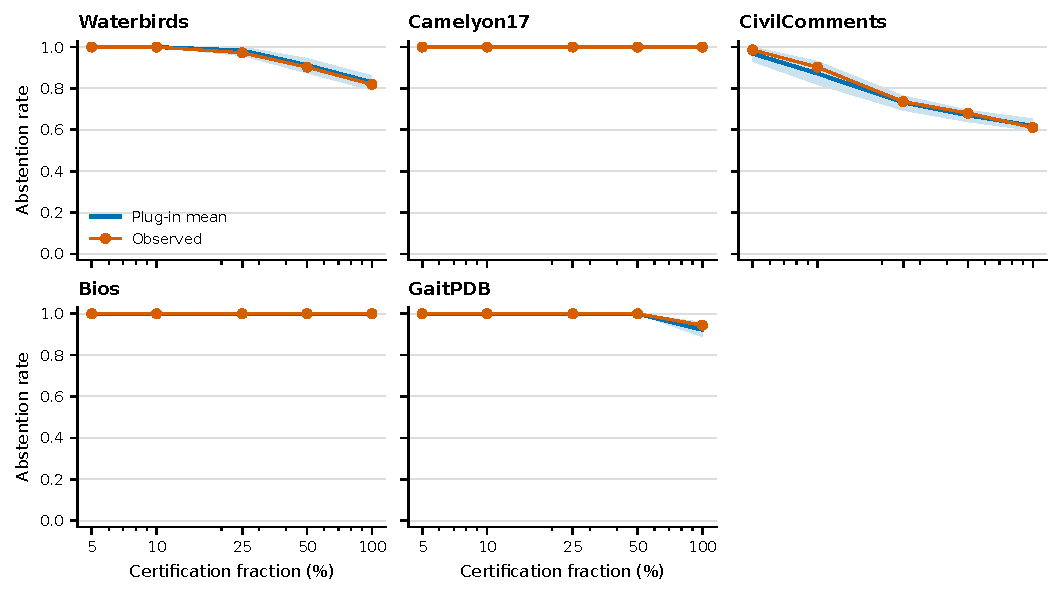
\includegraphics[width=0.96\textwidth]{../../figures/vera_real_learning_curve.pdf}
\caption{Observed real-data abstention versus a full-certification empirical
plug-in bootstrap. Resampling preserves registered strata and aligned
dependence across candidates and attackers. Unlike Fig.~\ref{fig:supp-exact},
this is a descriptive calibration diagnostic because the same full
certification fold estimates its bootstrap law.}
\label{fig:supp-real-learning}
\end{figure*}
}{}

\section{Official Real-Study Protocol}

The real study crosses INLP, R-LACE, LEACE, TaCo, and MANCE++ with Waterbirds,
Camelyon17-WILDS, CivilComments-WILDS, Bios, and GaitPDB at untouched seeds
5--12. Candidate construction uses at most 8,000 eraser-training examples and 2,000 construction
examples; certification and external evaluation each use at most 8,000
examples. Standardization and randomized PCA are fitted on eraser-training data
only. Every edit retrains a balanced logistic target probe and four leakage
attackers: linear logistic, RBF-Nystroem logistic, random forest, and a two-layer
MLP.

The registered grid uses certification fractions
$\{0.05,0.10,0.25,0.50,1.00\}$, paired target-harm thresholds
$\tau\in\{0.05,0.10,0.20\}$, leakage thresholds
$\lambda\in\{0.60,0.70,0.80\}$, $\delta=0.05$, primary budget $\Gamma=1$,
shifted sensitivity $\Gamma=1.01$, and radius cap $\Gamma_{\max}=8$. The
decision rules are always deploy, point-feasible validation selection,
VERA-IUT, the VERA simultaneous envelope, and an external oracle used only for
evaluation.

Camelyon17 center 2 is absent from certification, while centers 0, 1, 3, and 4
are observed. Its center-0-versus-other binary source label is constant in the
center-2 external slice. The primary protocol therefore assigns center 2 a
zero envelope coordinate and abstains for a declared five-center deployment.
This is procedural non-certifiability, not by itself a measured external
contract violation.

\section{Statistical Integrity}

Threshold pairs and nested fractions share the same eight seed-level fits and
examples. Configuration-level Clopper--Pearson and McNemar calculations are
retained as preregistered diagnostics, not treated as independent-trial
inference. The primary comparison averages each rule's nine outcomes within
seed and applies the preregistered exact one-sided sign-flip test over eight
seed blocks, with Holm correction over four externally estimable datasets.
All adjusted values are reported regardless of outcome. Seeds 0--4 contribute
to none of these estimates or tests.

External labels are unused by edit construction and candidate selection.
The unattended runner nevertheless computes external arrays run by run after
each candidate is fixed; aggregate analysis is deferred until the entire
official matrix and receipt audit finish. The paper does not claim that
external labels were physically inaccessible throughout execution.

\IfFileExists{vera_supplement_results.tex}{
  \section{Receipt-Level Confirmatory Results}
\begin{table*}[t]
\centering\scriptsize
\begin{tabular}{llrrrr}
\toprule
Dataset & Rule & Deploy & Viol./estimable & Cond. viol. & Unsupported \\
\midrule
Bios & Always deploy & 72/72 & 71/72 & 98.6\% & 0 \\
Bios & Point selection & 0/72 & 0/72 & NA & 0 \\
Bios & VERA-IUT & 0/72 & 0/72 & NA & 0 \\
Bios & VERA envelope & 0/72 & 0/72 & NA & 0 \\
Bios & External oracle & 1/72 & 0/72 & 0.0\% & 0 \\
\addlinespace
Camelyon17-WILDS & Always deploy & 72/72 & 0/0 & NA & 72 \\
Camelyon17-WILDS & Point selection & 23/72 & 0/0 & NA & 23 \\
Camelyon17-WILDS & VERA-IUT & 0/72 & 0/0 & NA & 0 \\
Camelyon17-WILDS & VERA envelope & 0/72 & 0/0 & NA & 0 \\
Camelyon17-WILDS & External oracle & 0/72 & 0/0 & NA & 0 \\
\addlinespace
CivilComments-WILDS & Always deploy & 72/72 & 42/72 & 58.3\% & 0 \\
CivilComments-WILDS & Point selection & 38/72 & 5/72 & 13.2\% & 0 \\
CivilComments-WILDS & VERA-IUT & 28/72 & 0/72 & 0.0\% & 0 \\
CivilComments-WILDS & VERA envelope & 27/72 & 0/72 & 0.0\% & 0 \\
CivilComments-WILDS & External oracle & 37/72 & 0/72 & 0.0\% & 0 \\
\addlinespace
GaitPDB & Always deploy & 72/72 & 3/72 & 4.2\% & 0 \\
GaitPDB & Point selection & 66/72 & 3/72 & 4.5\% & 0 \\
GaitPDB & VERA-IUT & 4/72 & 0/72 & 0.0\% & 0 \\
GaitPDB & VERA envelope & 0/72 & 0/72 & NA & 0 \\
GaitPDB & External oracle & 72/72 & 0/72 & 0.0\% & 0 \\
\addlinespace
Waterbirds & Always deploy & 72/72 & 50/72 & 69.4\% & 0 \\
Waterbirds & Point selection & 38/72 & 6/72 & 15.8\% & 0 \\
Waterbirds & VERA-IUT & 13/72 & 0/72 & 0.0\% & 0 \\
Waterbirds & VERA envelope & 9/72 & 0/72 & 0.0\% & 0 \\
Waterbirds & External oracle & 36/72 & 0/72 & 0.0\% & 0 \\
\addlinespace
\bottomrule
\end{tabular}
\caption{Full-size primary results. Each dataset has $8\times9=72$ threshold--seed configurations per rule. Unsupported counts flag deployment into the registered Camelyon17 support mismatch; they are not recoded as measured violations.}
\end{table*}

\begin{table*}[t]
\centering\scriptsize
\begin{tabular}{lrrrrr}
\toprule
Dataset & Point-only & VERA-only & Sign-flip Holm & Sign-test Holm & McNemar Holm \\
\midrule
Bios & 0 & 0 & 1.0000 & 1.0000 & 1.0000 \\
CivilComments-WILDS & 5 & 0 & 0.5000 & 0.5000 & 0.1875 \\
GaitPDB & 3 & 0 & 1.0000 & 1.0000 & 0.5000 \\
Waterbirds & 6 & 0 & 0.5000 & 0.5000 & 0.1250 \\
\bottomrule
\end{tabular}
\caption{Inference diagnostics. Sign-flip is the preregistered seed-blocked test. The sign test is a symmetry-free, lower-power secondary sensitivity. McNemar counts share fits and thresholds and are descriptive only. All values are Holm-adjusted over the four externally estimable datasets.}
\end{table*}

Safe-retention uncertainty: seed-cluster bootstrap 95\% interval 27.5\%--34.5\%; configuration-level Clopper--Pearson diagnostic 23.5\%--39.0\%. The maximum supported dataset--seed VERA violation rate was 0.0\%.

\begin{table}[t]
\centering\small
\begin{tabular}{lrr}
\toprule
Official eraser & Candidate points & Run receipts \\
\midrule
INLP & 4 & 40 \\
LEACE & 1 & 40 \\
MANCE++ & 1 & 40 \\
RLACE & 2 & 40 \\
TaCo & 4 & 40 \\
\midrule
Total & 12 & 200 \\
\bottomrule
\end{tabular}
\caption{Every candidate is generated by pinned official upstream code. One run receipt contains the complete registered strength frontier for one dataset, method, and seed; there are no proxy rows.}
\end{table}

}{
  \section{Receipt-Level Results}
  The locked official matrix and fail-closed aggregate analysis are still in
  progress in this source state. No placeholder value is a scientific result.
}

\IfFileExists{vera_ablation_results.tex}{
  \section{Secondary Sensitivity Analyses}
\begin{table*}[t]
\centering\scriptsize
\begin{tabular}{llrrr}
\toprule
Dimension & Condition & Deploy & Measured violation & Safe retention \\
\midrule
fixed profile shift budget & gamma=1 & 12.5\% & 0.0\% & 30.8\% \\
fixed profile shift budget & gamma=1.01 & 10.3\% & 0.0\% & 25.3\% \\
fixed profile shift budget & gamma=1.05 & 4.4\% & 0.0\% & 11.0\% \\
fixed profile shift budget & gamma=1.1 & 0.6\% & 0.0\% & 1.4\% \\
fixed profile shift budget & gamma=1.25 & 0.0\% & 0.0\% & 0.0\% \\
fixed profile shift budget & gamma=1.5 & 0.0\% & 0.0\% & 0.0\% \\
fixed profile shift budget & gamma=2 & 0.0\% & 0.0\% & 0.0\% \\
fixed profile shift budget & gamma=4 & 0.0\% & 0.0\% & 0.0\% \\
\addlinespace
attacker portfolio & drop\_forest & 12.5\% & 0.0\% & 30.8\% \\
attacker portfolio & drop\_linear & 13.1\% & 0.0\% & 32.2\% \\
attacker portfolio & drop\_mlp & 25.0\% & 14.9\% & 32.2\% \\
attacker portfolio & drop\_rbf & 12.8\% & 0.0\% & 31.5\% \\
attacker portfolio & full & 12.5\% & 0.0\% & 30.8\% \\
attacker portfolio & linear\_only & 43.6\% & 34.0\% & 40.4\% \\
attacker portfolio & linear\_rbf & 27.2\% & 17.7\% & 32.2\% \\
\addlinespace
eraser frontier & all five official erasers & 12.5\% & 0.0\% & 30.8\% \\
eraser frontier & leave INLP out & 8.9\% & 0.0\% & 29.4\% \\
eraser frontier & leave LEACE out & 12.2\% & 0.0\% & 30.1\% \\
eraser frontier & leave MANCE++ out & 12.5\% & 0.0\% & 30.8\% \\
eraser frontier & leave R-LACE out & 12.5\% & 0.0\% & 31.2\% \\
eraser frontier & leave TaCo out & 9.2\% & 0.0\% & 25.4\% \\
\addlinespace
frontier granularity & coarse\_5 & 11.4\% & 0.0\% & 31.8\% \\
frontier granularity & full\_12 & 12.5\% & 0.0\% & 30.8\% \\
\addlinespace
\bottomrule
\end{tabular}
\caption{Outcome-blindly locked secondary analyses. External safety always uses all four attackers. Candidate alpha and envelope multiplicity remain fixed at the original 12-candidate family, so removing attackers or erasers receives no confidence-allocation windfall.}
\label{tab:ablations}
\end{table*}

}{}

\section{Claim Boundary}

VERA does not prove perfect erasure, security against every measurable
attacker, fairness for unmeasured concepts, clinical safety, or validity on new
support. The density-ratio budgets are declared sensitivity parameters, not
facts estimated from an external test set. Internal audits check consistency
and provenance but cannot establish novelty, proof correctness, or conference
acceptance. Two cold reviews from researchers who publish in machine learning
remain a mandatory submission gate.
